\section{The K-mer Representation Quality} \label{sec:K_mer_Representation}

Investigation on the anomalies resulted in two persistent clustering errors \autoref{fig:PCA_Cluster_Knee_4} \textbf{\textsf{B}} and \textbf{\textsf{D}}. To evaluate if the method is suitable for the clustering of \gls{IAV} possible error sources are discussed.

% \begin{figure}[!hbt]
%     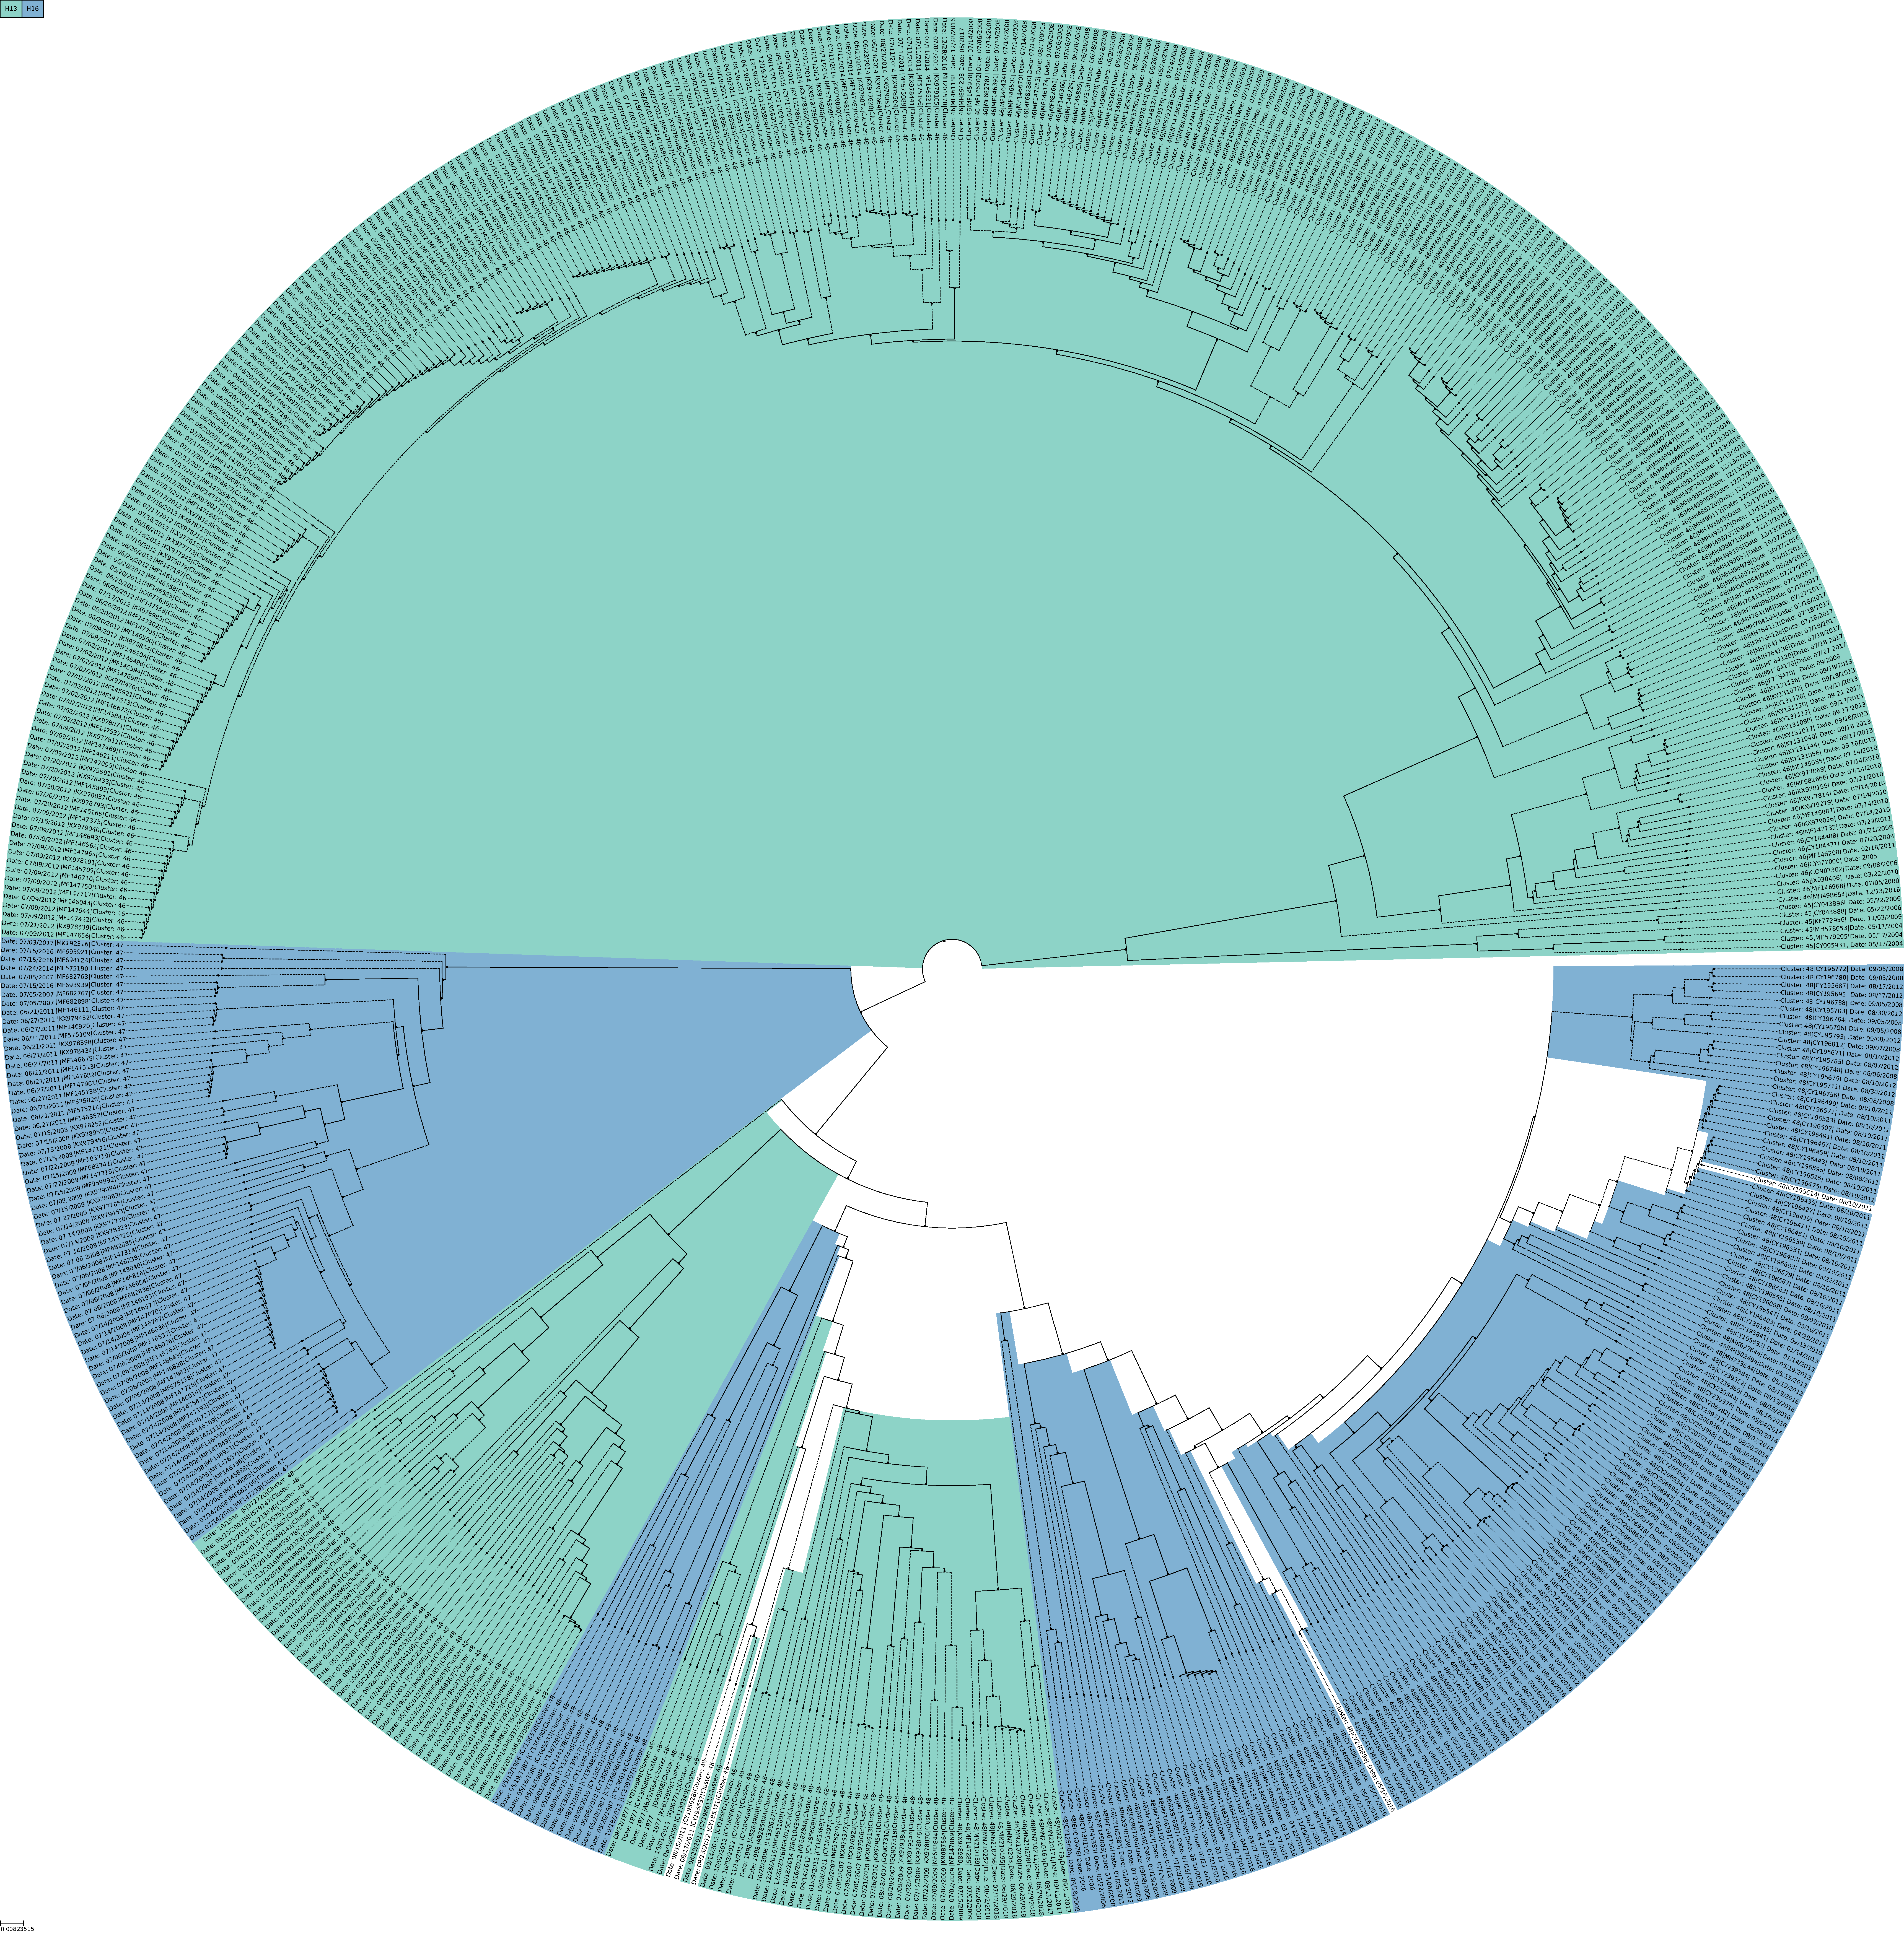
\includegraphics[width=\dimexpr\textwidth-2\fboxsep-2\fboxrule,fbox]{PCA/Clustertree_Segment_4_H_Knee_Zoom.pdf}
%     \caption[H13/H16 Simple Clustering Example with \Acrshort{PCA}]{\textbf{H13/H16 Simple Clustering Example with \Acrshort{PCA}.} .}
%     \label{fig:PCA_Clusteree_Knee_Zoom}
% \end{figure}

% \begin{figure}[!hbt]
%     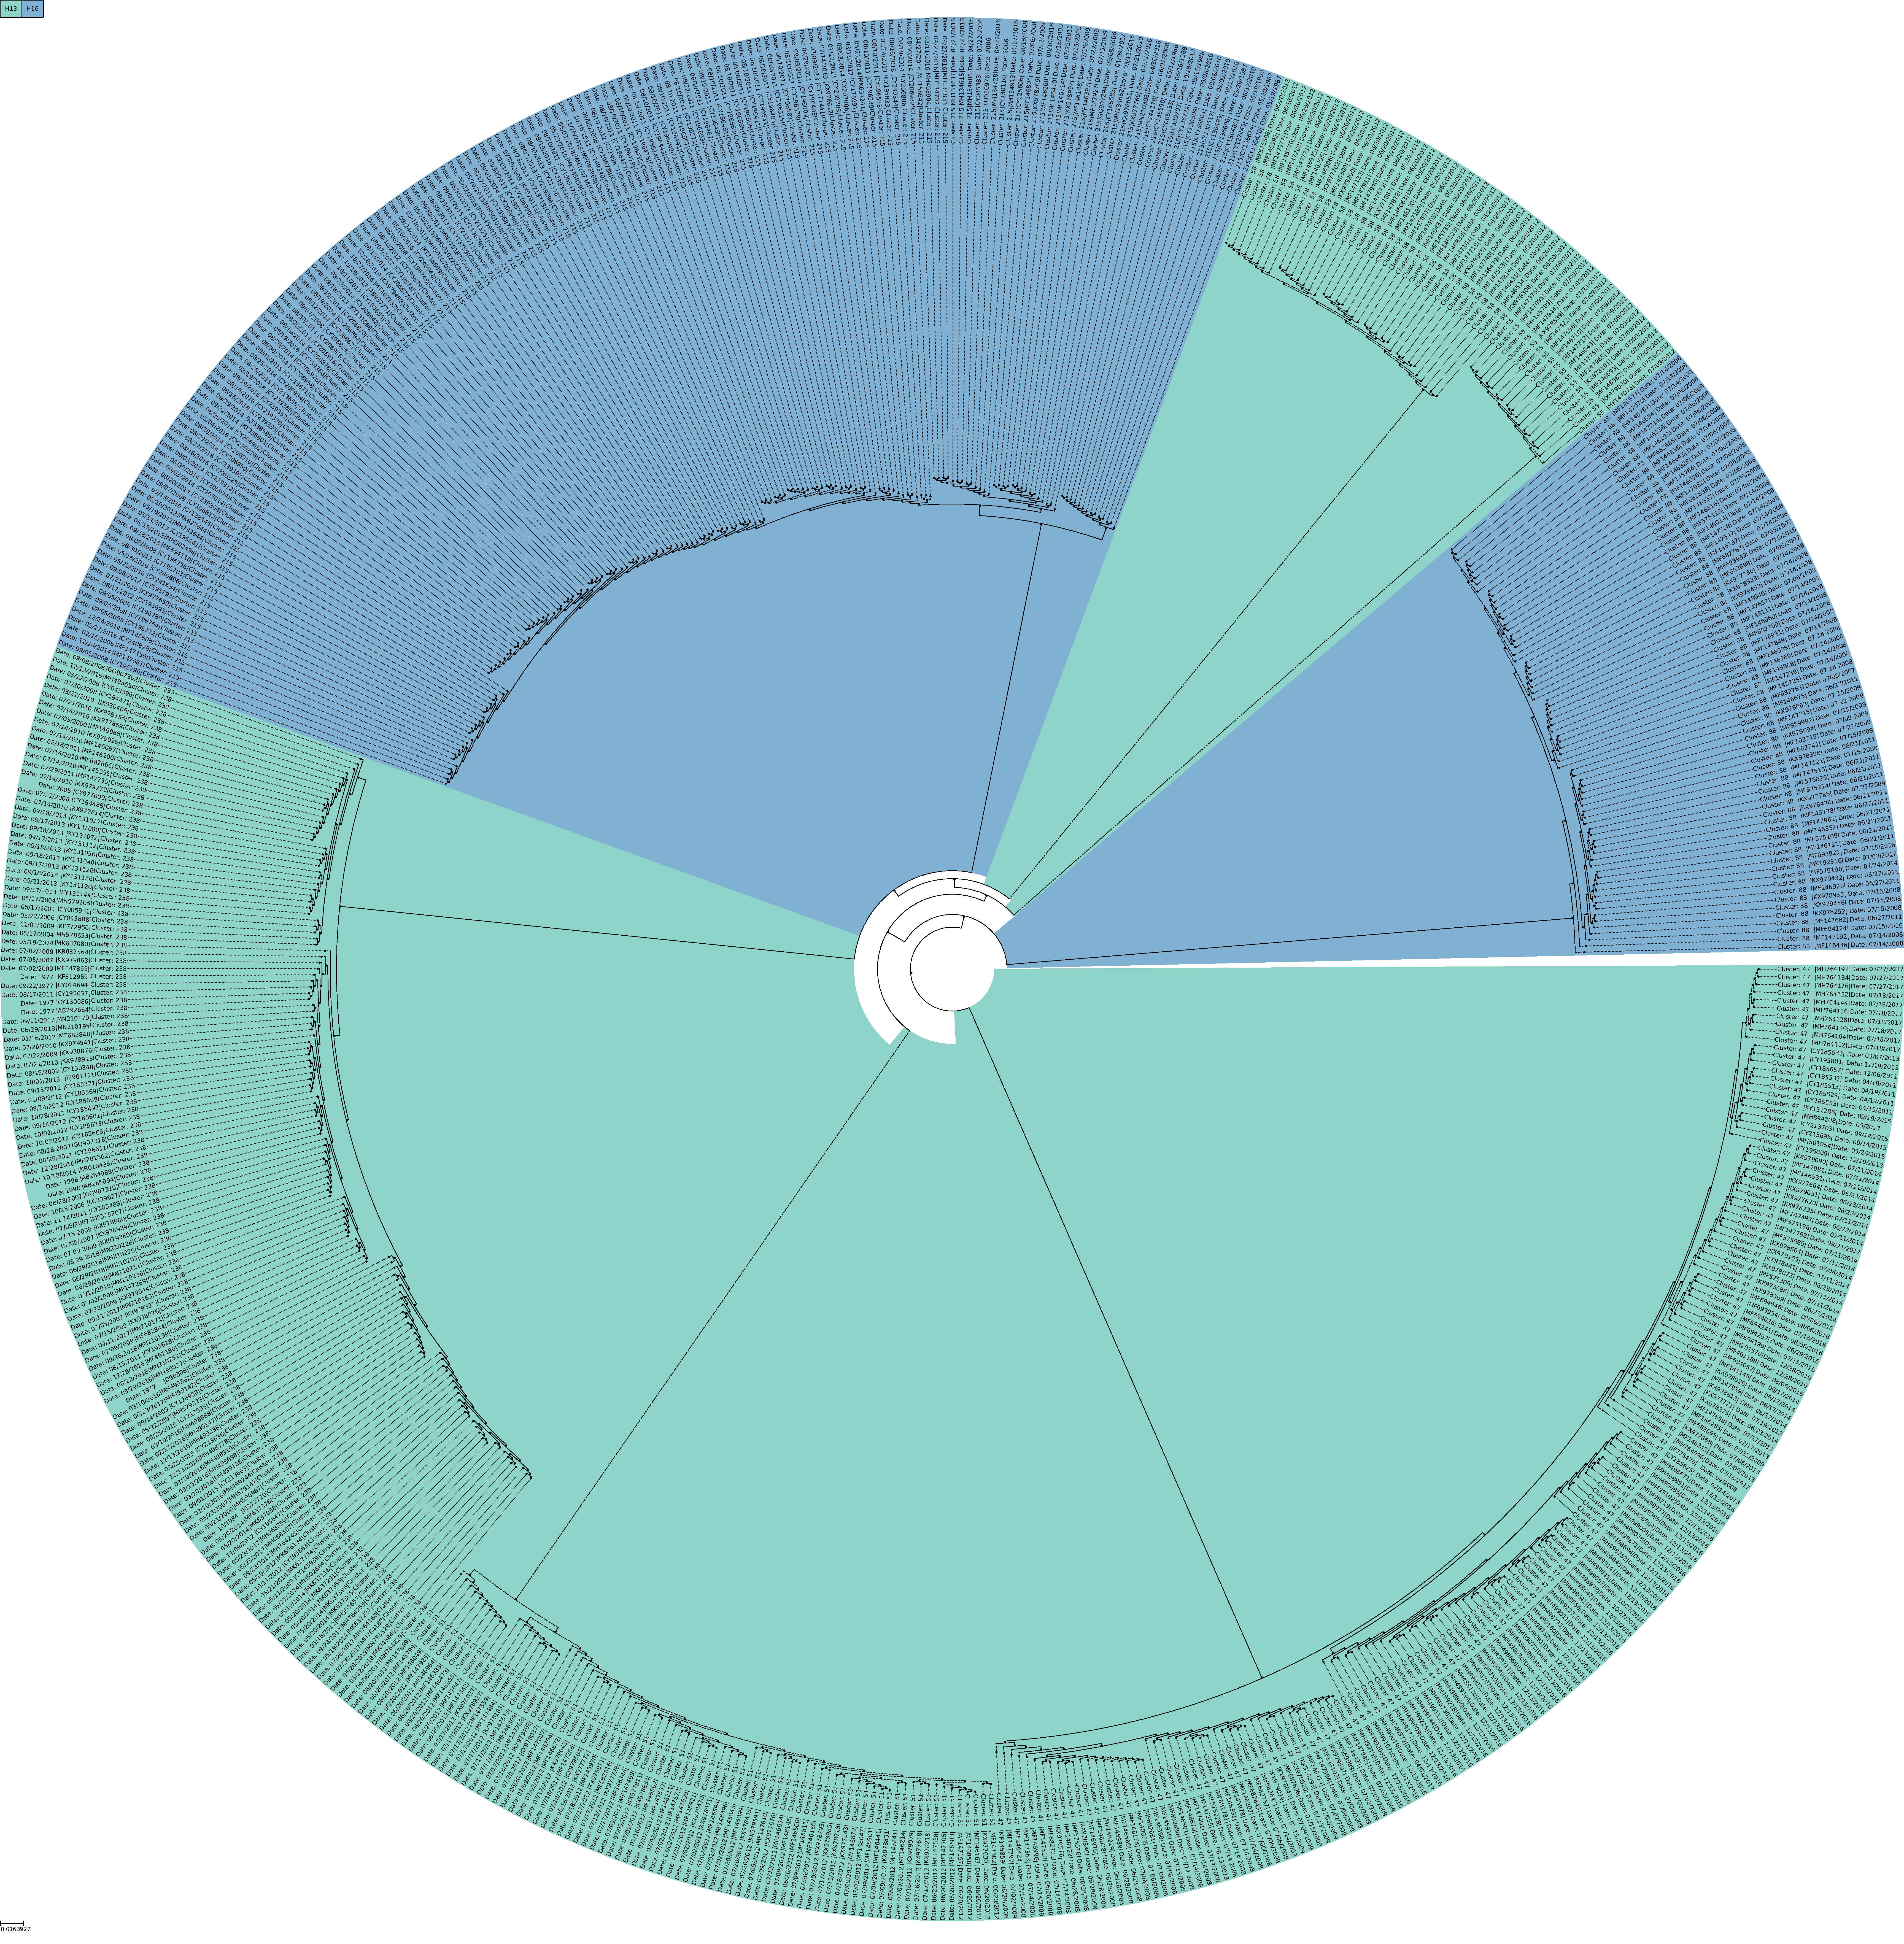
\includegraphics[width=\dimexpr\textwidth-2\fboxsep-2\fboxrule,fbox]{UMAP/Clustertree_Segment_4_H_Knee_Zoom.pdf}
%     \caption[H13/H16 Simple Clustering Example with \Acrshort{UMAP}]{\textbf{H13/H16 Simple Clustering Example with \Acrshort{UMAP}.} .}
%     \label{fig:UMAP_Clusteree_Knee_Zoom}
% \end{figure}

% \begin{figure}[!hbt]
%     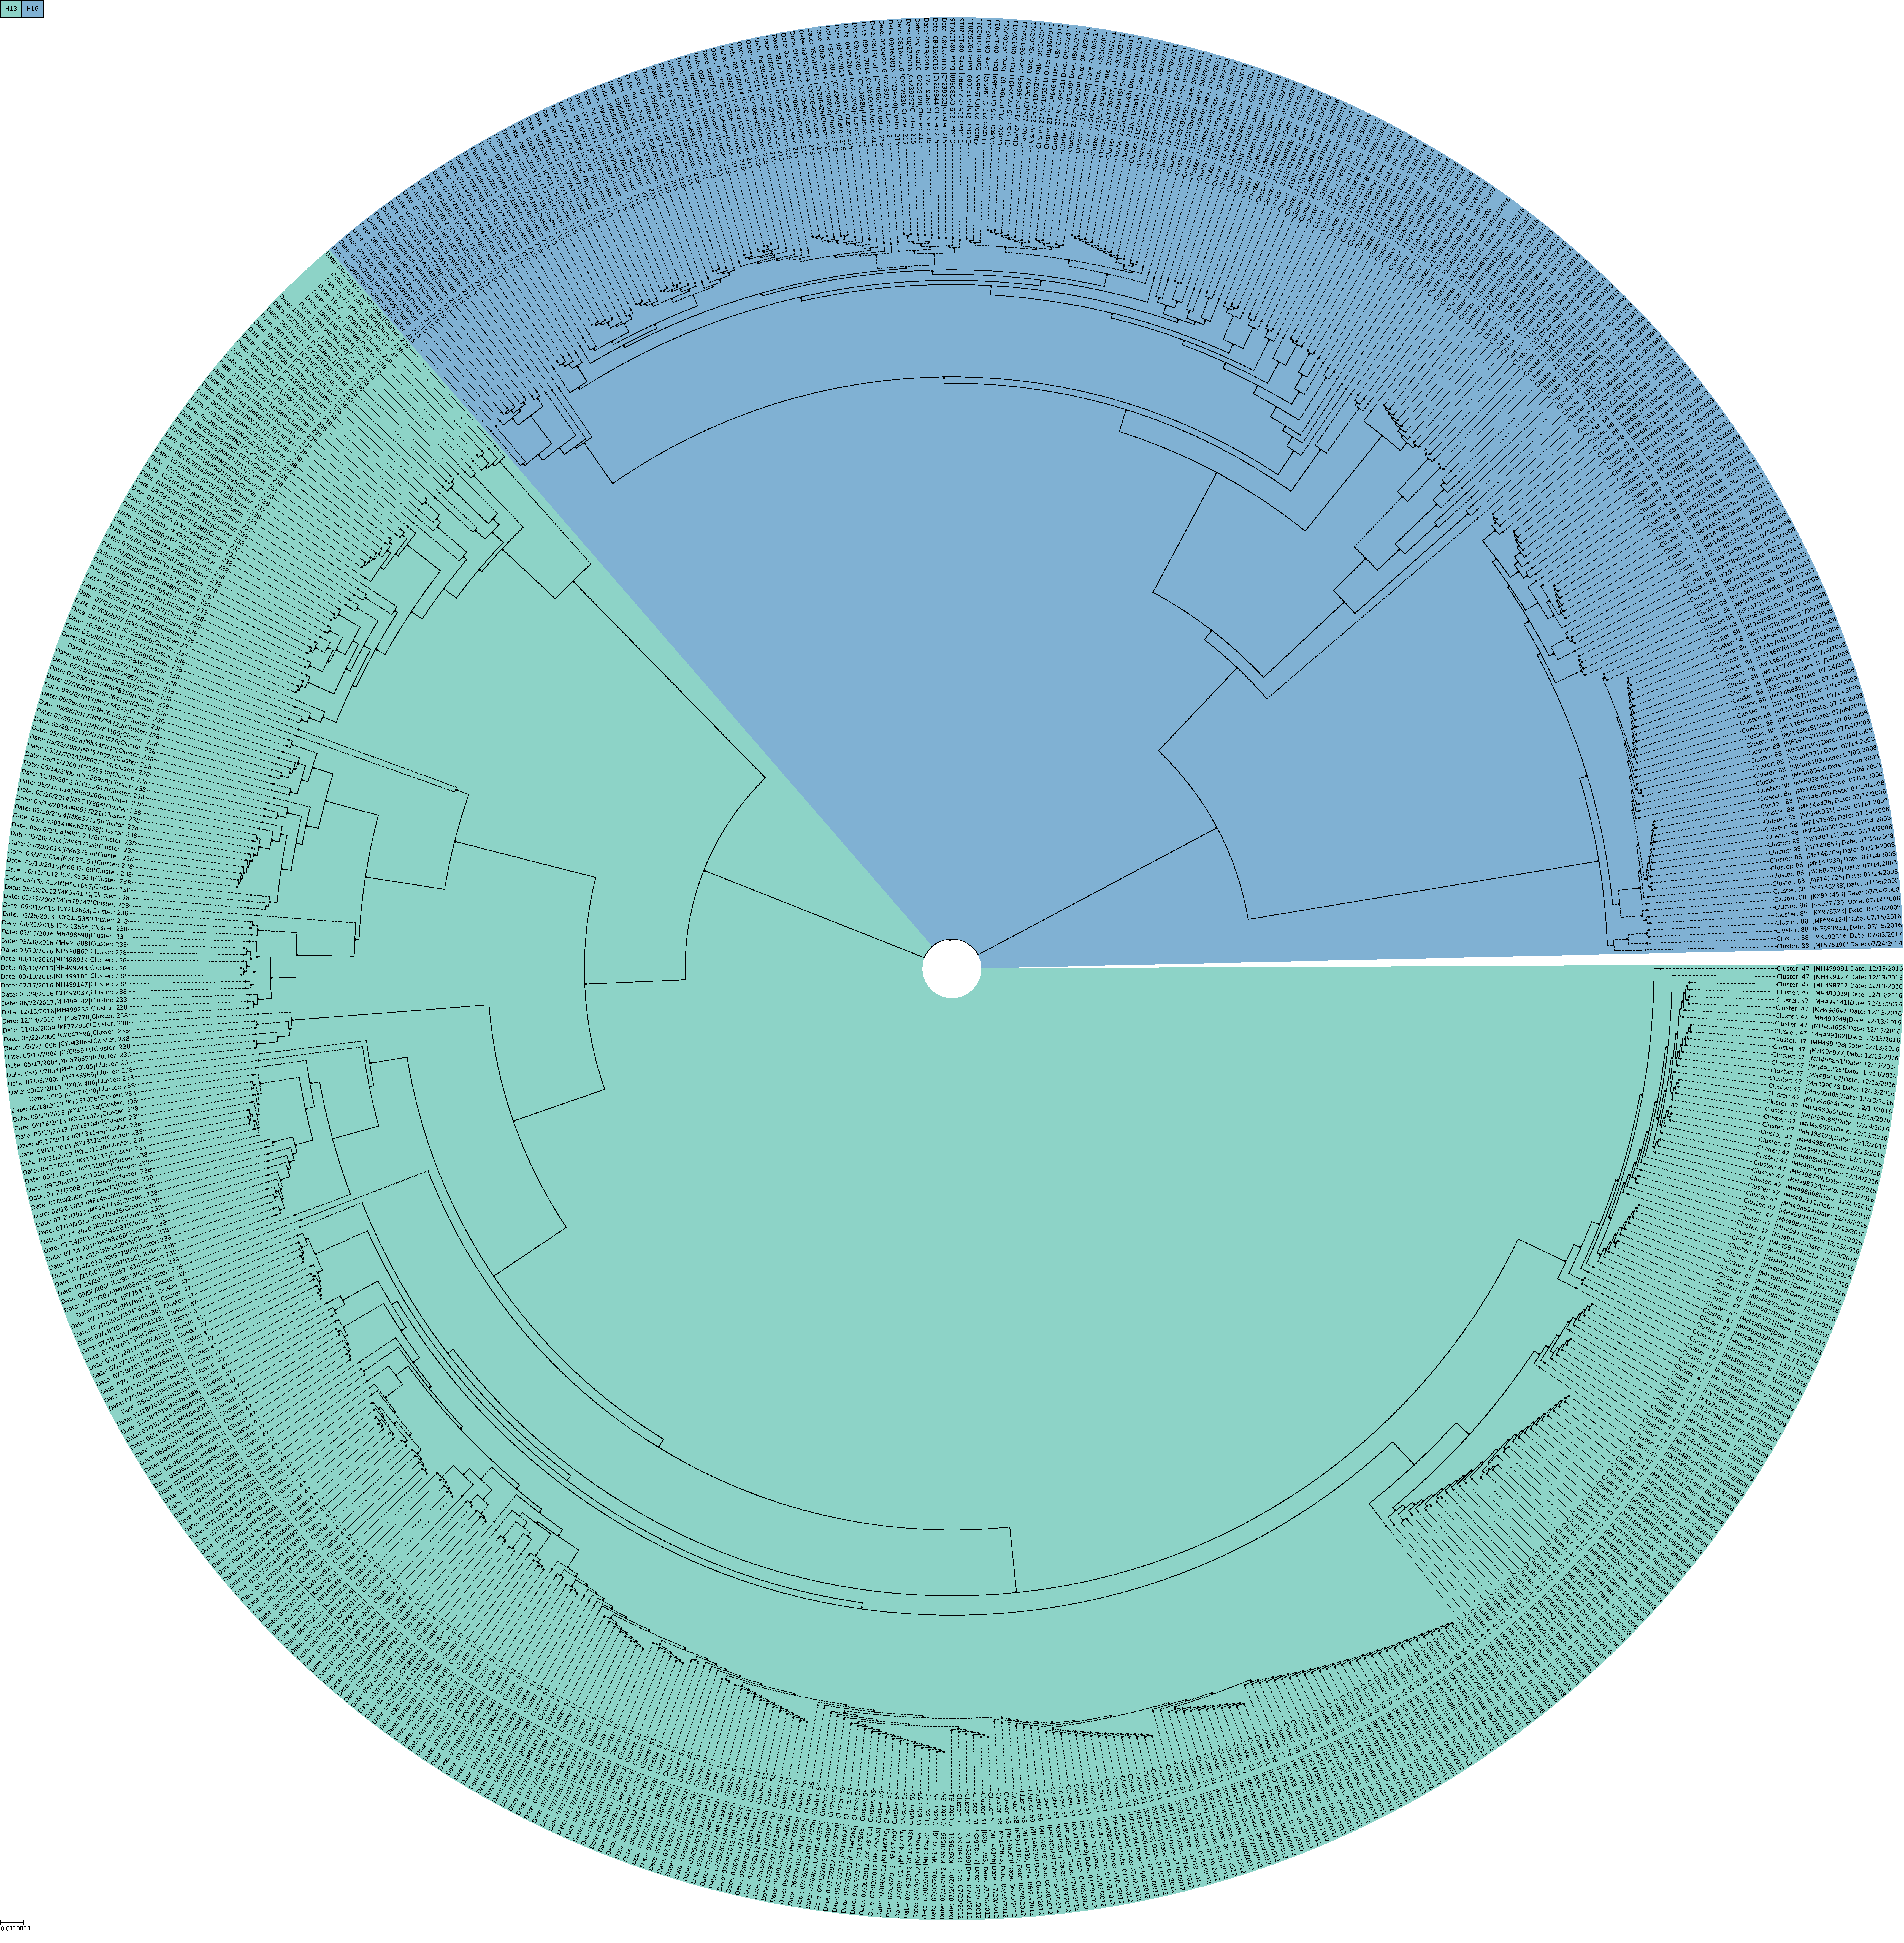
\includegraphics[width=\dimexpr\textwidth-2\fboxsep-2\fboxrule,fbox]{UMAP/Guidetree_Segment_4_H_Focus.pdf}
%     \caption[H13/H16 Simple Clustering Example with \Acrshort{MSA}]{\textbf{H13/H16 Simple Clustering Example with \Acrshort{MSA}.} .}
%     \label{fig:Guidetree_Focus}
% \end{figure}

\begin{figure}[hbt]
    \centering
    \begin{tikzpicture}
        \node[anchor=south west,inner sep=0] (image) at (0,0) {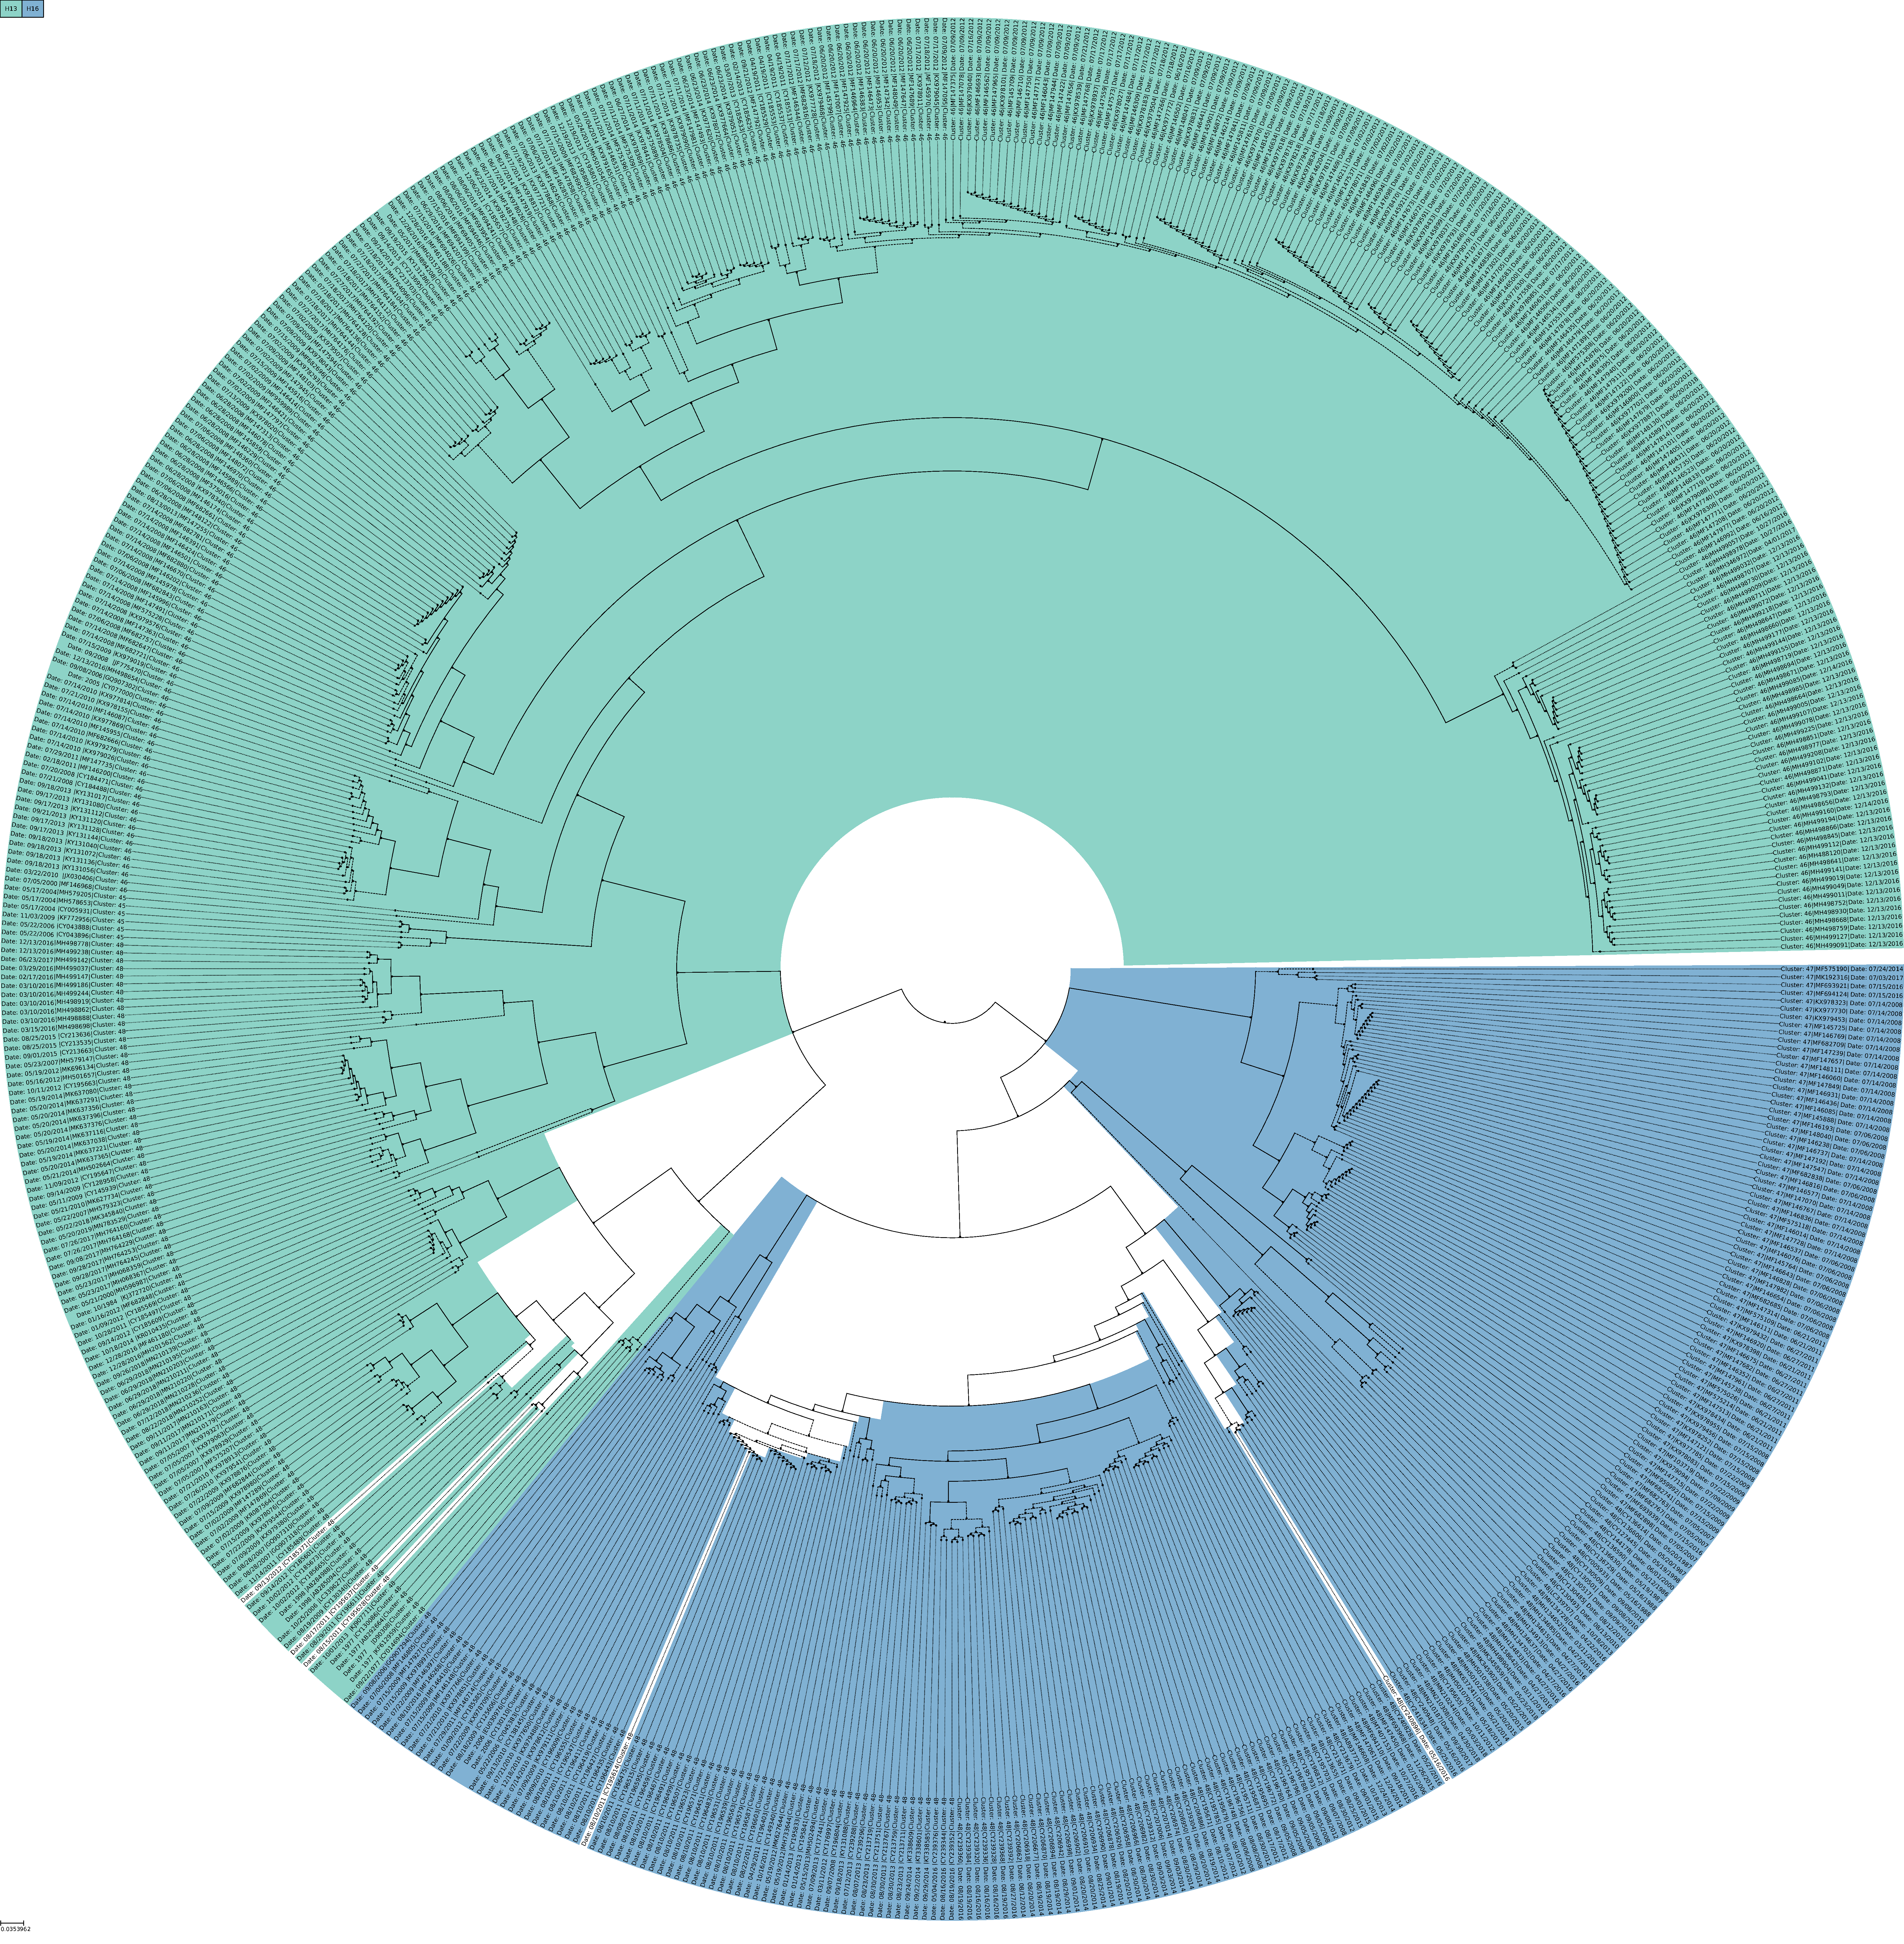
\includegraphics[width=\textwidth]{PCA/Precalculated_Segment_4_H_Cosine.pdf}};
        \begin{scope}[x={(image.south east)},y={(image.north west)}]
            %\draw[help lines,xstep=.1,ystep=.1] (0,0) grid (1,1);
            \draw[draw = none, fill = white] (0,1) rectangle (0.1,0.9);
            \draw[draw = none, fill = white] (0,0) rectangle (0.1,0.1);
            \draw[draw = black, thick, fill = black, fill opacity=0.0] (0.754,0.750) rectangle (0.999,0.505);
            \node at (0.754, 0.505) [fill=Red!80,thick,shape=circle,draw=black,inner sep=2pt] {\textbf{\textsf{C}}};
            %\draw[draw = black, thick, fill = black, fill opacity=0.2] (0.344, 0.603) rectangle (0.589,0.358);
            %\node at (0.344, 0.358) [fill=Red!80,thick,shape=circle,draw=black,inner sep=2pt] {\textbf{\textsf{A}}};
            \node at (0.425,0.525) [arrowstyle=1.5cm, arrowfillR, anchor=east, rotate=270] {\textbf{\textsf{A}}};
            \node at (0.55,0.525) [arrowstyle=1.5cm, arrowfillR, anchor=east, rotate=270] {\textbf{\textsf{B}}};
            %\draw[|-|] (0.975,0.5035) arc[start angle=0,end angle=170,radius=0.475, thick] node[midway,fill=Red!80,thick,shape=circle,draw=black,inner sep=2pt] {\textbf{\textsf{D}}};
            %\node at (0.5,0.505) [shape = circle,inner sep=140pt, fill = black] {};
            \node at (0.31,0.595) [arrowfillG, arrowstyle=1.5cm, anchor=east, rotate=315] {46};
            \node at (0.305,0.51) [arrowfillG, arrowstyle=1.5cm, anchor=east, rotate=45] {45};
            \node at (0.6,0.5) [arrowfillG, arrowstyle=1.5cm, anchor=east, rotate=225] {\rotatebox{180}{47}};
            \node at (0.35,0.455) [arrowfillG, arrowstyle=1.5cm, anchor=east, rotate=90] {48};
            \node at (0.425,0.42) [arrowfillG, arrowstyle=1.5cm, anchor=east, rotate=90] {48};
            \node at (0.54,0.435) [arrowfillG, arrowstyle=1.5cm, anchor=east, rotate=135] {\rotatebox{180}{48}};
        \end{scope}
    \end{tikzpicture}
    \caption[H13/H16 Precalculated \Acrshort{UPGMA} Tree (cosine)]{\textbf{H13/H16 Precalculated \Acrshort{UPGMA} Tree (cosine).} .}
    \label{fig:Precalculated_Cosine}
\end{figure}

By building a \gls{UPGMA} tree on the non reduced segment 4 k-mer frequency vectors of the H13 and H16 subtypes, the unbiased relation of sequences from these subtypes can be analyzed (\autoref{sec:MAFFT}). Also the fundamental use of k-mer frequencies can be validated or rejected. Not colored sequences are unclassified sequences (\autoref{fig:Frequency_4}) that also can't be assigned to a subtype, since they were clustered in a inconclusive cluster. Therefore these sequences are unclassified sequences from cluster 48 (\autoref{fig:PCA_Clusteree_Knee_4} \textbf{\textsf{B}}).

\begin{figure}[hbt]
    \centering
    %\begin{adjustbox}{minipage=\dimexpr\textwidth-2\fboxsep-2\fboxrule,fbox}
    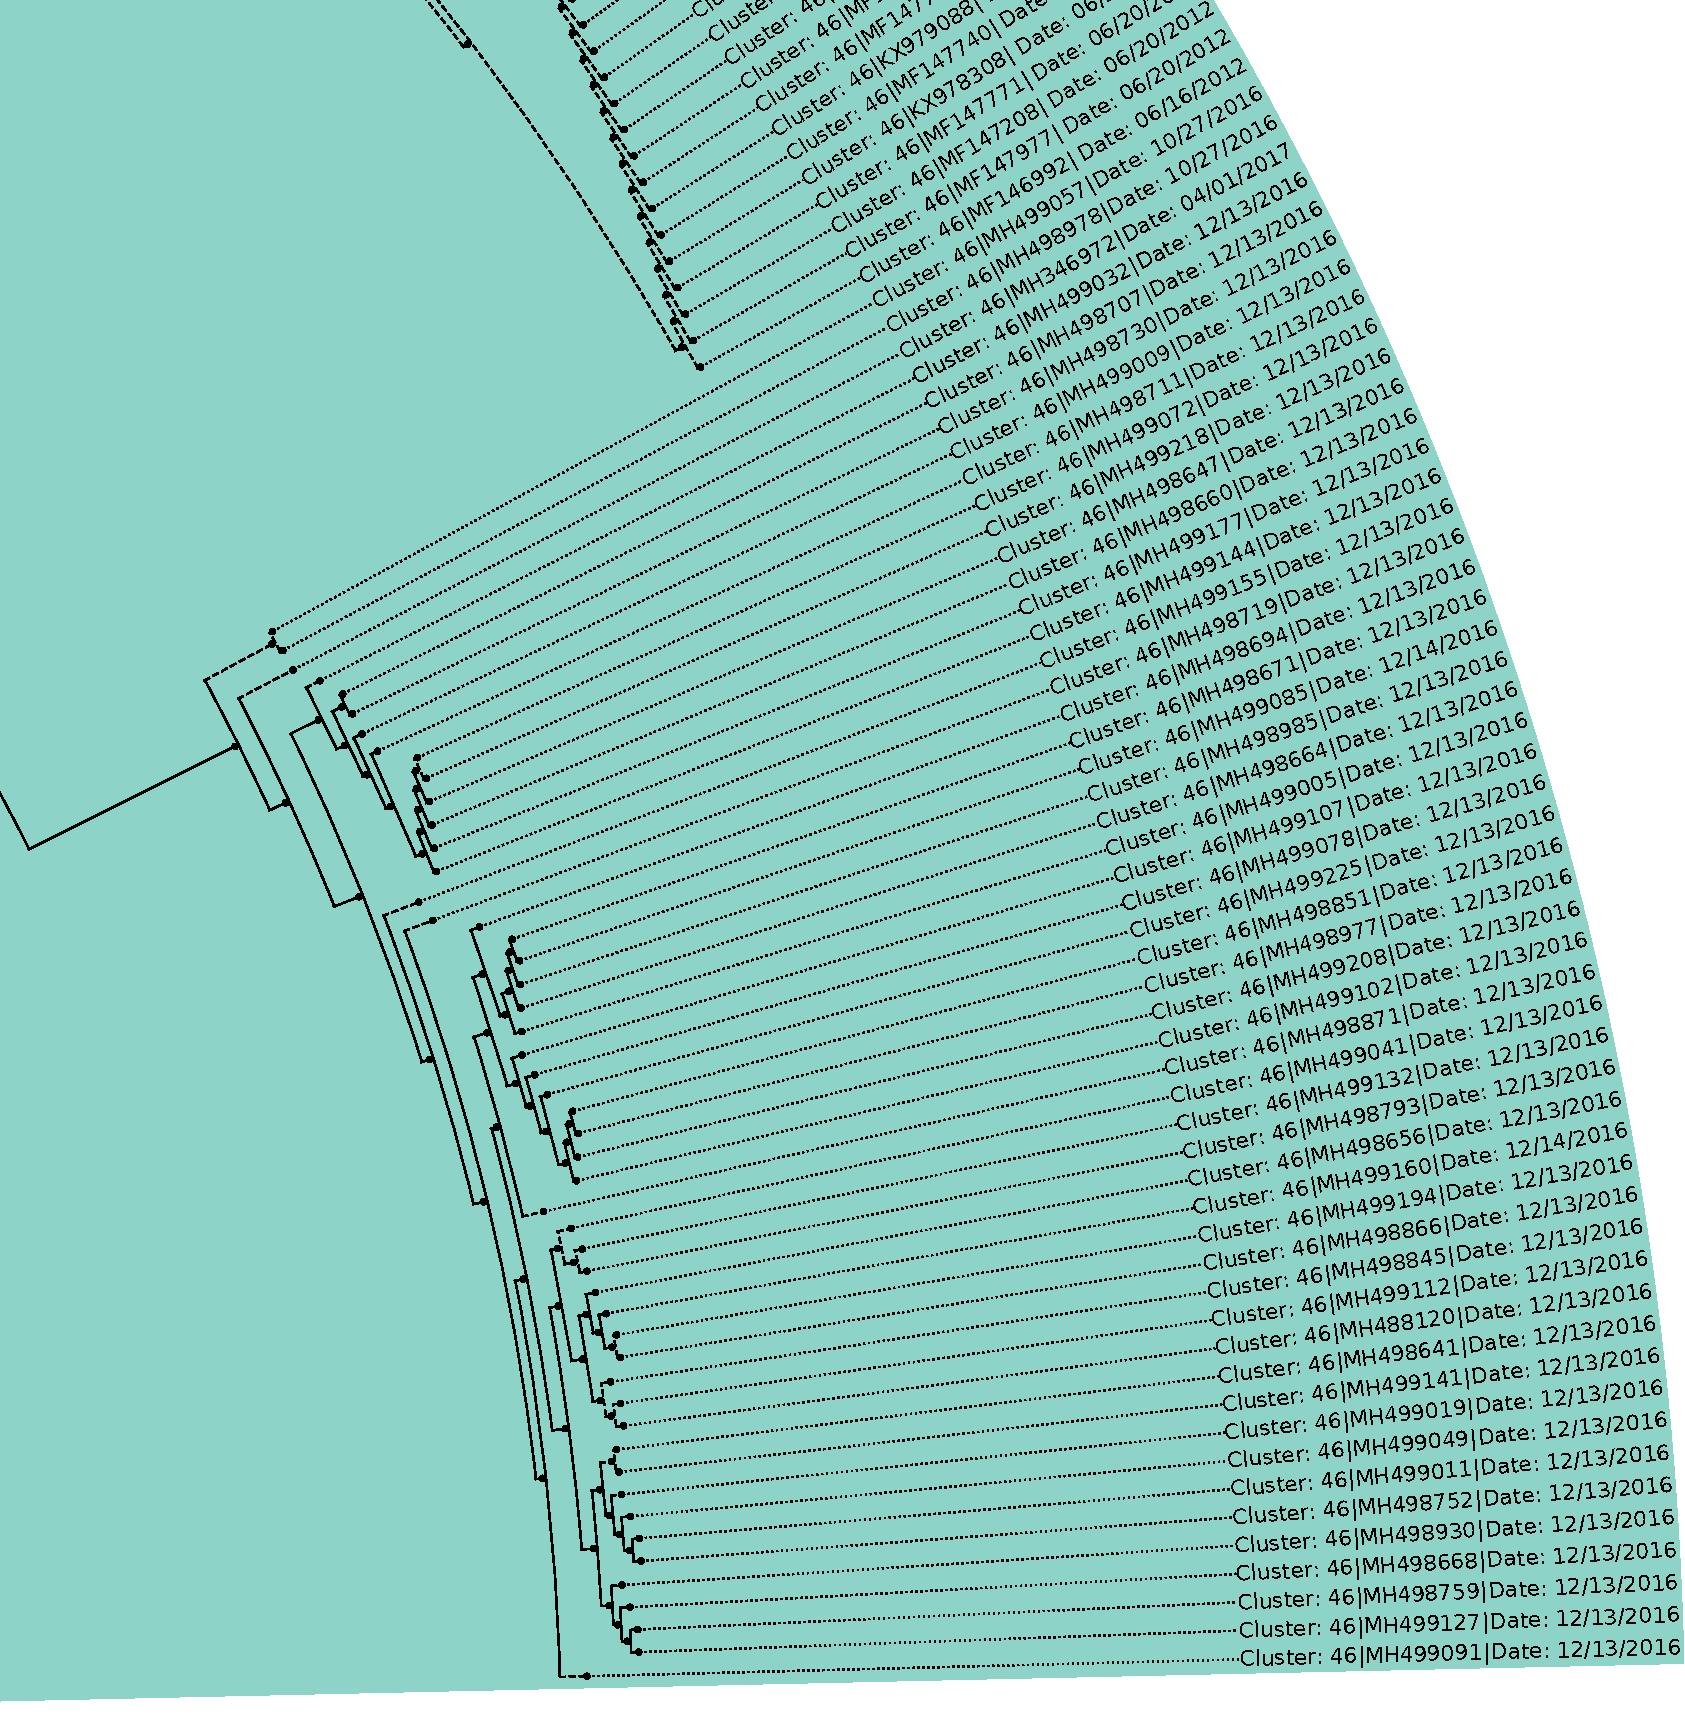
\includegraphics[width=\textwidth]{Graphics/identical.pdf}
    \caption[Focus in Precalculated \Acrshort{UPGMA} Tree]{Focus in Precalculated \Acrshort{UPGMA} Tree}
    \label{fig:focus}
\end{figure}

While both subtypes in \autoref{fig:Precalculated_Cosine} are completely seperated directly after the trees root, there are also subdivisions for both subtypes directly after. This early subdivision can point to the existence of more subtle variations with major difference to each other than the existing subtype classification reveals. In this case it appears as if at least two sub groups for H13 and at least two or three subgroups for H16 exist. The threshold is difficult to define here and no clustering was performed in this case so this statement is based only on the early subdivision in the k-mer \gls{UPGMA}-tree (\autoref{fig:Precalculated_Cosine} \textbf{\textsf{A}} and \textbf{\textsf{B}}). The exact seperation from the root is in line with the centroid guide-tree based on \gls{MSA} were both subtypes are completeley seperated to (\autoref{fig:PCA_Guidetree_Centroid_4}). Since this is also in line with the subtype classification the k-mer frequency seems to work for this project. Furthermore when focusing on a portion of the \gls{UPGMA}-tree with very small difference from sequence to sequence in \autoref{fig:Precalculated_Cosine} \textbf{\textsf{C}} the similar collection date of all these sequences (12/13/2016) stand out. The only sequences not from this collection date but nevertheless included in this subtree are MH499057, MH498978, MH346972, MH499085 and MH499160. Two of the tree are from the same collection date but some days prior to the rest, while the third was collected some days after the 12/13/2016. The three sequences are the last linked sequences in the subtree with the highest distance in comparison to the rest and their collection date is nearly the same as for the rest. The last two sequences with different date MH499085 and MH499160 are in the middle of the subtree but the collected just one day after the rest. This points in the direction that even small differences are noticed by the k-mer approach. The collection date was used as comparison here because many of the sequences in the subtree have very different strain names but are very or completely similar and therby cause a misinterpretation. Example for this case are MH499085 of strain A/environment/Chile/C20369/2016 and MH498671 of strain A/white\_backed\_stilt/Chile/C20090/2016. There strain names differ drastically as the virus was collected apparently completely different but the sequenced genomes are in fact 100\% the same. Around the tree in nearly every case similar collection dates have a small distance based on the k-mer frequency supporting the statement of the usability of k-mer frequencies for \gls{IAV} clustering. Same calculation for th precalculated \gls{UPGMA} tree was also repated with euclidean distance and can be found in the \autoref{chap:Appendix}.

%frage is hier welche Methode die bessere representation ausstrahlt, sprich UMAP vgl. precalc ja/nein? dann PCA vgl precalc passt? ja/nein?